\documentclass[10pt]{article}
\usepackage[margin=0.85in]{geometry}
\usepackage{amsmath,amssymb}
\usepackage[T1]{fontenc}
\usepackage[utf8]{inputenc}
\usepackage{lmodern}
\usepackage{microtype}
\usepackage{enumitem}
\usepackage{booktabs}
\usepackage{graphicx}
\usepackage{url}
\usepackage[hidelinks]{hyperref}
\hypersetup{pdftitle={A Strong-Field Turn-Off for the Quadrature MOND Kernel: Planetary Safety, a Finite Vacuum Term, and the Offset Reading}, pdfauthor={The authors}}
\setlist{nosep,leftmargin=1.3em}
\setlength{\parskip}{3pt}\setlength{\parindent}{0pt}
\sloppy
\newcommand{\fpath}[1]{\nolinkurl{#1}}
\begin{document}

\begin{center}
{\Large\bfseries A Strong-Field Turn-Off for the Quadrature MOND Kernel:\\ Planetary Safety, a Finite Vacuum Term, and the Offset Reading}\\[6pt]
{\small The authors --- 2026-10-05, version 1.0 --- AI-assisted research programme; not peer reviewed}
\end{center}

% Every number below is produced by a committed script: sonnet55_push/puzzle_32pi/p35_kernel_tail_fix.py (SPARC, planets, vacuum; 4/4, MUTATE fails 3),
% make_paper41_figures.py (PAPER41_figures_numbers.json) and the lanes cited in place. PAPER41_audit.py checks the tagged numbers against those files.

\begin{abstract}
\noindent The quadrature law $g^2=g_N^2+a_0g_N$, i.e.\ $\nu(y)=\sqrt{1+1/y}$ with $y=g_N/a_0$ (Milgrom 1999, eq.~9), has a slow strong-field tail, $\nu-1\simeq 1/(2y)$. Held to all accelerations it gives a constant anomalous acceleration $a_0/2$ in the Solar System, 1279 times the Earth--Mars ephemeris bound, and it makes the vacuum term of the theory's field Lagrangian (QUMOND, or the nonrelativistic limit of bimetric MOND) diverge linearly. We replace the tail by $\nu_{\rm fix}(y)=1+(\sqrt{1+1/y}-1)/[1+(y/y_t)^2]$, which equals the law below a turn-off $y_t$ and falls as $y^{-3}$ above it. On SPARC the fixed kernel is indistinguishable from the exact law for $y_t\ge100$ ($|\Delta\chi^2|\le1.06$ on about 3000 points); every planet passes for $y_t\le7.7\times10^5$ (Mars binds); the vacuum term becomes finite, $\Lambda/a_0^2\simeq(\pi/4)\,y_t$. The repair costs one constant. If, in addition, the vacuum energy of the $a_0$ sector is the observed dark energy (the ``offset reading'', an input), $y_t$ is fixed: $128.9$ on the footing that defines $a_0$ from $\Lambda$, and $94$--$103$ for measured $a_0=1.05$--$1.10\times10^{-10}$\,m\,s$^{-2}$, i.e.\ the boost turns off at $g_N\approx10^{-8}$\,m\,s$^{-2}$, at the upper edge of present rotation-curve data. The turn-off value depends on its shape ($k=3,4$ give 167.5 and 182.4 on the framework footing), so it is not a derivation of the coefficient $\kappa=\tfrac12$, which stays fitted.
\end{abstract}
% AUDIT: A01

\section{The problem}
The law $g_{\rm obs}^2=g_N^2+a_0g_N$ fits the radial acceleration relation of SPARC galaxies [LMS16] and is the deep-MOND relation with the next-order term of Milgrom's 1999 vacuum construction [M99]. Its interpolating function has $\nu-1\simeq1/(2y)$ for $y\gg1$, the ``$\alpha=1$'' tail. Two consequences follow, and both are failures of the law held at all accelerations, not of its galaxy-scale content:
\begin{itemize}
\item \textbf{Planets.} The anomalous acceleration $(\nu-1)g_N\to a_0/2$ is a constant $4.7\times10^{-11}$\,m\,s$^{-2}$ toward the Sun, 1279 times the Earth bound $3.66\times10^{-14}$\,m\,s$^{-2}$ and comparably over Mars [SJ06, M09]. Sereno \& Jetzer require a tail exponent $\gtrsim1.5$.
\item \textbf{Vacuum term.} In QUMOND, or in the $\alpha+\beta=0$ bimetric theory whose nonrelativistic limit it is [M09b, eq.~3], the field Lagrangian leaves a constant when the field vanishes. With no constant in strong fields this gives $\Lambda/a_0^2=\tfrac12\int_0^\infty2y(\nu-1)\,dy$ [M09b, eq.~24 with $f(1)=1$], the same in the exchange-symmetric bimetric class by an exact boundary-term identity (programme lane p25). For $\nu=\sqrt{1+1/y}$ the integral grows linearly with any cutoff; cut at the Planck acceleration it gives $\Lambda=\tfrac12a_0a_P/c^4$, about $10^{59}$ times the observed value (p27).
\end{itemize}
% AUDIT: A02

\section{The turn-off}
We keep the law where it is measured and switch the tail off above $y_t$:
\begin{equation}
\nu_{\rm fix}(y)=1+\frac{\sqrt{1+1/y}-1}{1+(y/y_t)^k},\qquad k=2\ \text{(default)} .
\end{equation}
Below $y_t$ this is the law (deep limit, landmark triplet and sum rule unchanged); above it $\nu-1\simeq y_t^k/(2y^{1+k})$. Figure~\ref{fig:tail} shows the fractional boost for three turn-offs against the planetary bounds converted to $\nu-1$.
\begin{figure}[h]\centering
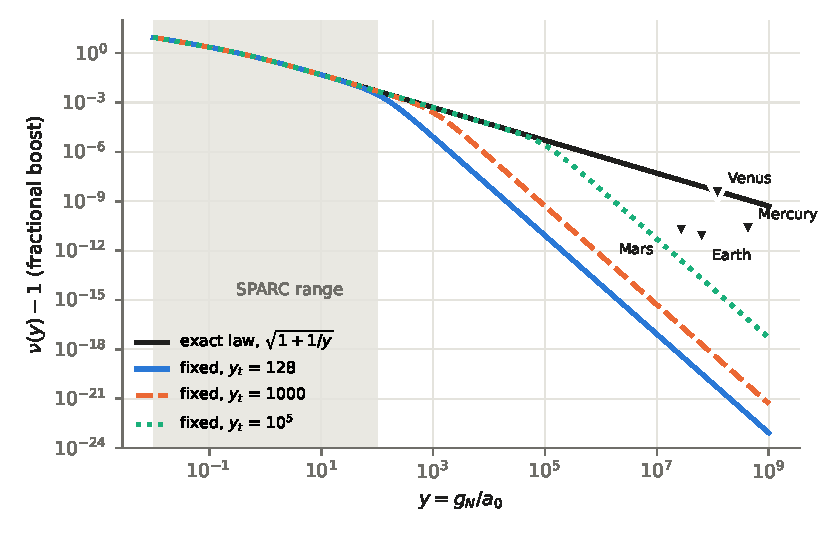
\includegraphics[width=0.78\textwidth]{fig1_paper41_tail.pdf}
\caption{Fractional boost $\nu-1$ against $y=g_N/a_0$. Black: the exact law. Coloured: the turn-off at $y_t=128$, $10^3$, $10^5$ (line style repeats the colour). Triangles: the planetary bounds on $\nu-1$ (bare, no external-field credit). Shaded: the SPARC range.}\label{fig:tail}
\end{figure}

\section{Results}
\textbf{Galaxies.} With the programme's SPARC profile likelihood (175 galaxies; $\Upsilon$ fixed at 0.5 with MLS16 cuts, or free per galaxy), the turn-off changes the best $\chi^2$ by $+0.07$, $+0.04$, $0.00$ (fixed $\Upsilon$) and $-1.06$, $-0.67$, $-0.01$ ($\Upsilon$ free) for $y_t=100$, 128, $10^3$: indistinguishable. A direct fit of $y_t$ bounds it only from below ($\Delta\chi^2<4$ for $y_t\ge20$ at fixed $\Upsilon$, $\ge2$ with $\Upsilon$ free; programme lane p36); the offset reading's values below change $\chi^2$ by less than 1.2.
% AUDIT: A03

\textbf{Planets.} The largest allowed turn-off is $y_t=7.7\times10^5$ (Mars), $1.77\times10^6$ (Earth), $5.4\times10^7$ (Mercury), $1.81\times10^8$ (Venus). At $y_t=128$ the worst planet sits at $2.8\times10^{-8}$ of its bound.
% AUDIT: A04

\textbf{Vacuum term.} The integral is finite: $\Lambda/a_0^2=77.85$, $99.81$, $784.4$ at $y_t=100$, 128, $10^3$ ($k=2$). To leading order it is $\tfrac12\int_0^\infty dy/[1+(y/y_t)^2]=(\pi/4)\,y_t$; the small-$y$ part of the kernel and a logarithm supply the rest (Fig.~\ref{fig:vac}).
% AUDIT: A05
\begin{figure}[h]\centering
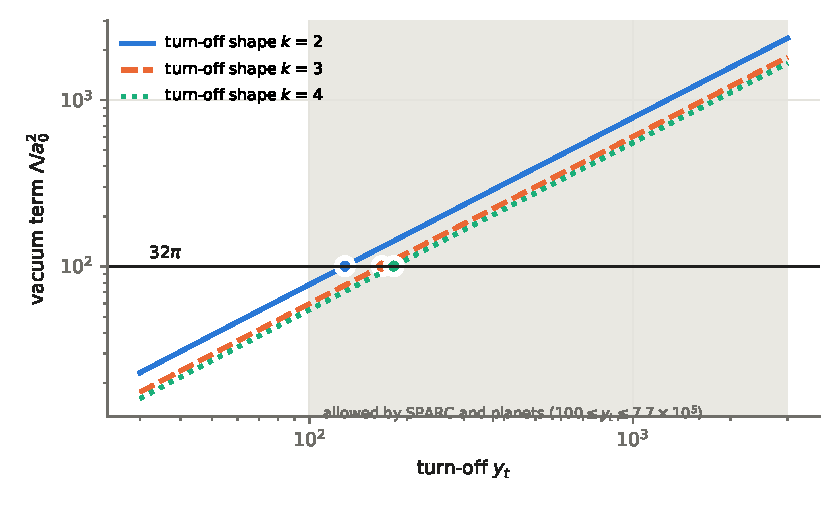
\includegraphics[width=0.78\textwidth]{fig2_paper41_vacuum.pdf}
\caption{The vacuum term $\Lambda/a_0^2$ against the turn-off $y_t$ for three turn-off shapes. Horizontal line: $32\pi$, the framework footing. Dots: where each shape meets it. Shaded: the window allowed by SPARC and the planets.}\label{fig:vac}
\end{figure}

\section{The offset reading}
If the $a_0$ sector's vacuum energy is the observed dark energy (an input; programme lane K), the turn-off is no longer free. Then $\Lambda_{\rm obs}/a_0^2$ fixes $y_t$:
\begin{center}
\begin{tabular}{lcc}
\toprule
$a_0$ (m\,s$^{-2}$) & $\Lambda_{\rm obs}/a_0^2$ & $y_t$ ($k=2$)\\
\midrule
$9.3603\times10^{-11}$ (defined from $\Lambda$, $\kappa=\tfrac12$) & 100.53 & 128.9\\
$1.05\times10^{-10}$ (MeerKAT MIGHTEE-HI) & 79.89 & 102.6\\
$1.0766\times10^{-10}$ (SPARC profile) & 75.99 & 97.6\\
$1.097\times10^{-10}$ (ensemble of nine analyses) & 73.19 & 94.1\\
\bottomrule
\end{tabular}
\end{center}
% AUDIT: A06
On measured $a_0$ the boost turns off at $y_t\approx94$--$103$, i.e.\ $g_N\approx10^{-8}$\,m\,s$^{-2}$, just at the upper edge of SPARC (about 5\% of points have $y>10$; the sample tops out near $y\approx110$). This is the reading's testable content: rotation-curve, lensing or dynamical data at $10\lesssim y\lesssim10^3$ (bulge-dominated inner regions, early-type galaxies) would see the boost fall below the exact law's by a factor $\approx1/[1+(y/y_t)^2]$. It also inherits lane K's consequence that with $w=-1$ the scale $a_0$ is constant in time. The companion paper develops this reading as a model of dark energy (doi:10.5281/zenodo.23171066).

\textbf{What it is not.} The turn-off value depends on the shape: $k=3$ and $k=4$ need $y_t=167.5$ and $182.4$ on the framework footing. The ``round'' 128 is $32\pi$ divided by the $\pi/4$ of the $k=2$ integral. The offset reading is a hypothesis, not a consequence of the action. Nothing here derives $\kappa=\tfrac12$ in $a_0=\kappa c\sqrt{G\rho_\Lambda}$.
% AUDIT: A07

\section{Summary}
A single turn-off removes the quadrature kernel's two strong-field failures (the planets and the divergent vacuum term) without touching galaxies, at the cost of one constant $y_t\in[100,\,7.7\times10^5]$. Under the offset reading that constant is set by $\Lambda/a_0^2$ and lands at the edge of current data, which makes it testable. The cold mass ($\Omega_ch^2\approx0.12$) is still required; no dark-matter particle is added.

\paragraph{Reproducibility.} \fpath{sonnet55_push/puzzle_32pi/p35_kernel_tail_fix.py} (4/4; the exact-law control fails 3), \fpath{qwen_claude_field_theory/papers_2026/make_paper41_figures.py}, \fpath{PAPER41_figures_numbers.json}, \fpath{PAPER41_audit.py}.

\small
\paragraph{References.}
[LMS16] Lelli, McGaugh \& Schombert, AJ 152, 157 (2016).
[M99] Milgrom, Phys.\ Lett.\ A 253, 273 (1999), astro-ph/9805346.
[M09] Milgrom, MNRAS 399, 474 (2009), arXiv:0906.4817.
[M09b] Milgrom, Phys.\ Rev.\ D 80, 123536 (2009), arXiv:0912.0790.
[SJ06] Sereno \& Jetzer, MNRAS (2006).
\end{document}
